\subsection{Relational games}

The \textit{relational games} dataset was contributed as a benchmark for relational reasoning by~\citep{shanahanExplicitlyRelationalNeural}. It consists of a family of binary classification tasks for identifying abstract relational rules between a set of objects represented as images. The objects consist of three sets of simple geometric shapes, referred to as ``pentominoes'', ``hexominoes'', and ``stripes''. The objects are arranged in a $3 \times 3$ grid. Each task corresponds to some relationship between the objects (see~\Cref{fig:relational_games_dataset}), and the target is to classify whether the relationship holds among a given sequence of objects or not.

In our experiments, we evaluate out-of-distribution generalization by training all models on the pentominoes objects and evaluating on the hexominoes and stripes objects. The input to all models is presented as a sequence of $9$ objects, each represented as a $12 \times 12 \times 3$ RGB image. In all models, the objects are processed independently by a CNN with a shared architecture. The individually-processed sequence of objects is then passed to the relation-processing component of the model. The results are then flattened and passed through an MLP with a shared architecture to produce the final prediction. We compare four models: a relational convolutional network (abbreviated RelConvNet), CoRelNet~\citep{kergNeuralArchitecture2022}, PrediNet~\citep{shanahanExplicitlyRelationalNeural}, and a Transformer~\citep{vaswani2017attention}. The architectural details of each model are described in~\Cref{tab:architectures} of the appendix.

The pentominoes split is used for training,
% We hold out 1000 samples for validation (during training) and 5000 samples for testing (after training), and use the rest as the training set. \awni{we don't show val or test accs on the pentos objects, so not relevant.}
and the hexominoes and stripes splits are used to test out-of-distribution generalization after training. We train for 50 epochs using the categorical cross-entropy loss and the Adam optimizer with learning rate $0.001$, $\beta_1 = 0.9, \beta_2 = 0.999, \epsilon = 10^{-7}$. We use a batch size of 512. For each model and task, we run 5 trials with different random seeds.

\begin{figure}
    \centering
    \begin{subfigure}[t]{0.37\textwidth}
        \centering
        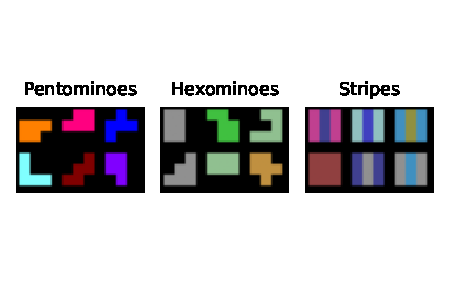
\includegraphics[width=0.9\textwidth]{figs/relational_games_objects.pdf}
        % \caption{Examples of objects from each split.}
        \label{fig:relational_games_objects}
    \end{subfigure}
    \begin{subfigure}[t]{0.62\textwidth}
        \centering
        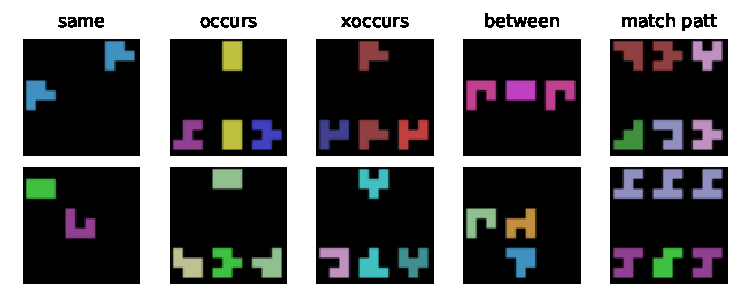
\includegraphics[width=0.9\textwidth]{figs/relational_games_tasks.pdf}
        % \caption{Examples of problem instances for each task. The top row is an example where the relation holds and the bottom row is an example where the relation does not hold.}
        \label{fig:relational_games_tasks}
    \end{subfigure}
    \caption{Relational games dataset.~\textbf{Left} Examples of objects from each split.~\textbf{Right} Examples of problem instances for each task. The first row is an example where the relation holds and the second row is an example where the relation does not hold.}\label{fig:relational_games_dataset}
\end{figure}


\begin{figure}
    \centering
    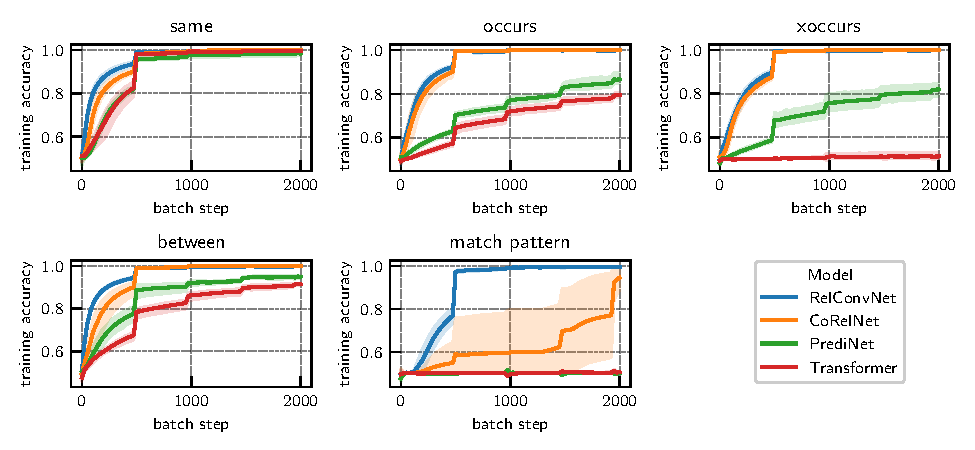
\includegraphics[width=0.9\textwidth]{figs/experiments/all_training_curves.pdf}
    \caption{Training curves, up to 2,000 batch steps, for each relational games task. Solid lines indicate the mean over 5 trials and the shaded regions indicate a bootstrap 95\% confidence interval.}\label{fig:training_curves}
    \vskip-20pt
\end{figure}

\textbf{Sample efficiency.} We observe that the relational inductive biases of RelConvNet, and relational models more generally, grant a significant advantage in sample-efficiency.~\Cref{fig:training_curves} shows the training accuracy over the first 2,000 batches for each model. RelConvNet, CoRelNet, and PrediNet are explicitly relational architectures, whereas the Transformer is not. The Transformer is able to process relational information through its attention mechanism, but this information is entangled with the features of individual objects (which, for these relational tasks, is extraneous information). The Transformer consistently requires the largest amount of data to learn the relational games tasks. PrediNet tends to be more sample-efficient. RelConvNet and CoRelNet are the most sample-efficient, with RelConvNet only slightly more sample-efficient on most tasks.

On the `match pattern' task, however, RelConvNet is significantly more sample-efficient. We attribute this to the fact that RelConvNet is able to model higher-order relations through its relational convolution module. The `match pattern' task can be thought of as a simple second-order relational task---it involves computing relations between two groups of objects, and comparing the relations within the two groups. The relational convolution module naturally models this kind of situation since learns representations of the relations among subsets of objects. %The performance we observe here indicates that the relational games dataset is in some sense saturated by models like RelConvNet and CoRelnet and that more complex relational benchmarks are needed to evaluate the limits of these models.

\begin{figure}
    \centering
    \begin{subfigure}{0.45\textwidth}
        \centering
        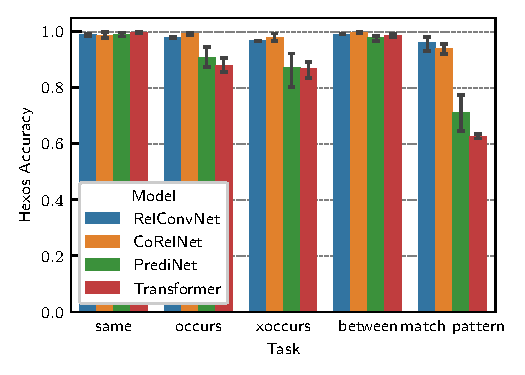
\includegraphics[width=0.9\textwidth]{figs/experiments/hexos_acc.pdf}
        \caption{OoD generalization on Hexos objects}\label{fig:ood_generalization_hexos}
    \end{subfigure}
    \begin{subfigure}{0.45\textwidth}
        \centering
        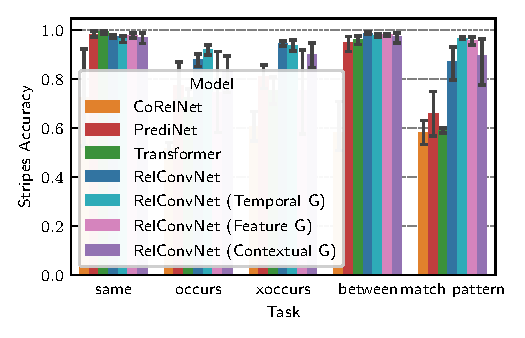
\includegraphics[width=0.9\textwidth]{figs/experiments/stripes_acc.pdf}
        \caption{OoD generalization on Stripes objects}\label{fig:ood_generalization_stripes}
    \end{subfigure}
    \caption{Out-of-distribution generalization on hold-out object sets. Bar heights indicate the mean over 5 trials and the errror bars indicate a bootstrap 95\% confidence interval.}\label{fig:ood_generalization}
    \vskip-10pt
\end{figure}

\textbf{Out-of-distribution generalization.}~\Cref{fig:ood_generalization} reports model performance on the two hold-out object sets after training. On the hexominoes objects, which are similar-looking to the pentominoes objects used for training, RelConvNet and CoRelNet do nearly perfectly. PrediNet and the Transformer do well on the simpler tasks, but struggle with the more difficult `match pattern' task. The stripes objects are visually more distinct from the training split objects, making generalization more difficult. We observe an overall drop in performance for all models. The drop is particularly dramatic for CoRelNet\footnote{Unlike~\citep{kergNeuralArchitecture2022}, we do not use temporal context normalization in our experiments. We believe this is the more appropriate choice for evaluating relational architectures such as RelConvNet and CoRelNet since TCN is an added confounder. We discuss this more in~\Cref{sec:appendix_tcn_discussion}.}. We conjecture that this is due to CoRelNet's inability to model multi-dimensional relations, necessitating that all relational information is squeezed into a scalar quantity. The separation between RelConvNet and the other models is largest on the ``match pattern'' task of the stripes split (the most difficult task and the most difficult generalization split). Here, RelConvNets maintain a mean accuracy of 87\% while the other models drop below 65\%. We attribute this to RelConvNet's natural ability to model higher-order relations as well as multi-dimensional relations.
